\documentclass[Nike]{tuberlinbeamer}

\usepackage[ngerman]{babel}  % 'babel' muss geladen werden
\usepackage[utf8]{inputenc}  % optional, aber empfehlenswert
\usepackage[square, numbers, comma, sort&compress]{natbib} 
\usepackage[absolute,overlay]{textpos}
\usepackage{multirow}
\usepackage{amsfonts}

% Die ueblichen Angaben
\title{Veranschaulichung digitaler Steuerprotokolle in der Lichttechnik}
\subtitle{Antrittsvortrag Bachelorarbeit}
\author[Conrad Klaus]{Conrad Klaus}
\institute{Fachgebiet Lichttechnik}

\newcommand{\customcite}[1]{
	\vskip0pt plus 1filll
	\color{grau}
	\raggedleft \tiny Bilder: \cite{#1}
}

\begin{document}

\begin{frame}
	\maketitle
\end{frame}
\begin{frame}{Agenda}
	\tableofcontents
\end{frame}


\section{Theoretischer Ansatz}

\begin{frame}{Theoretischer Ansatz}
   \begin{tabular}{cl}  
		\begin{tabular}{c}
				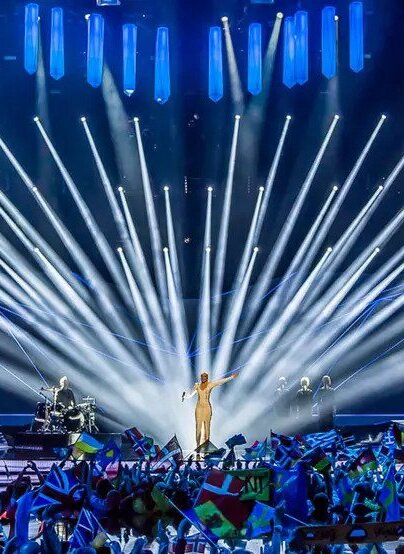
\includegraphics[height=\textheight - 13pt]{pictures/dmx-demo}
		\end{tabular}
		& \parbox{0.5\linewidth}{
			\emph{DMX Protokoll}
			\begin{itemize}
				\item Digital Multiplex (DMX) steuert Leuchten
				\item Farbe, Helligkeit, Ausrichtung etc.
				\item 512 Kanäle mit Wertebereich 0-255
			\end{itemize}
			\vspace{3ex}
			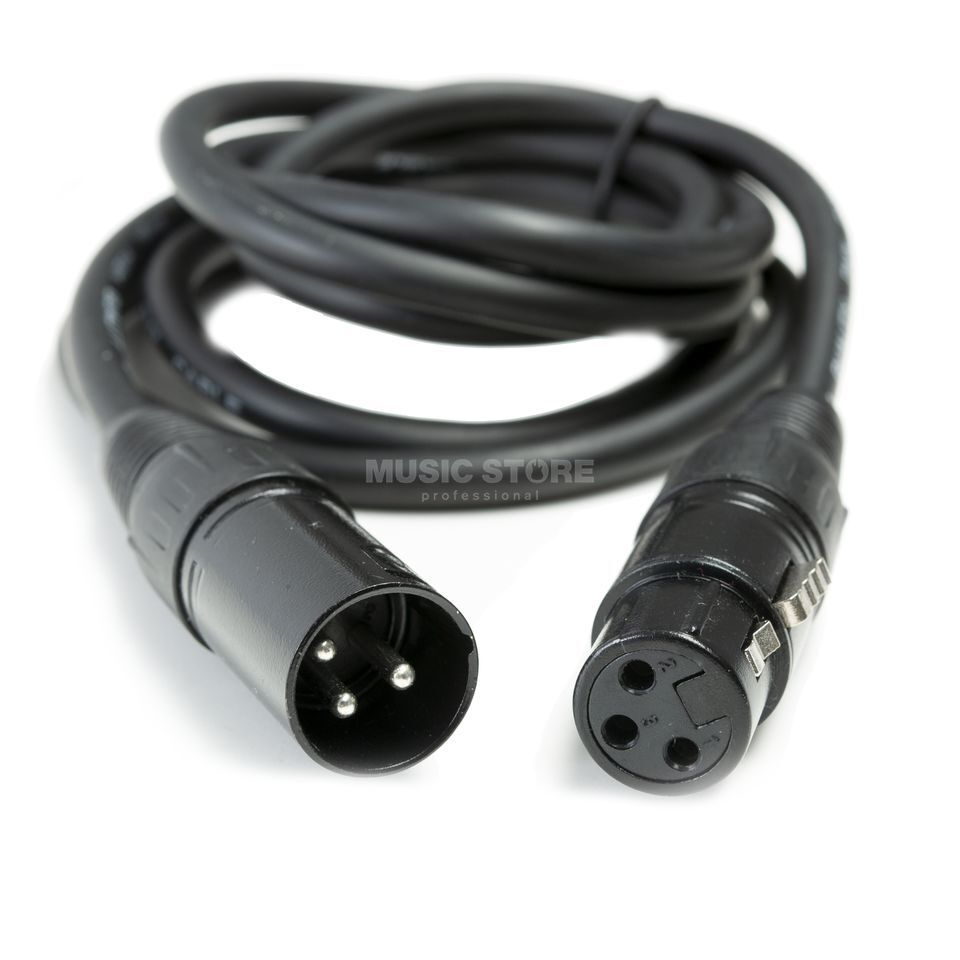
\includegraphics[scale= 0.1]{pictures/dmx-cable}
		}
	\end{tabular}
	\customcite{dmx_demo, dmx_cable}
\end{frame}
\begin{frame}{Theoretischer Ansatz}
	\begin{tabular}{cl}  
		\begin{tabular}{c}
			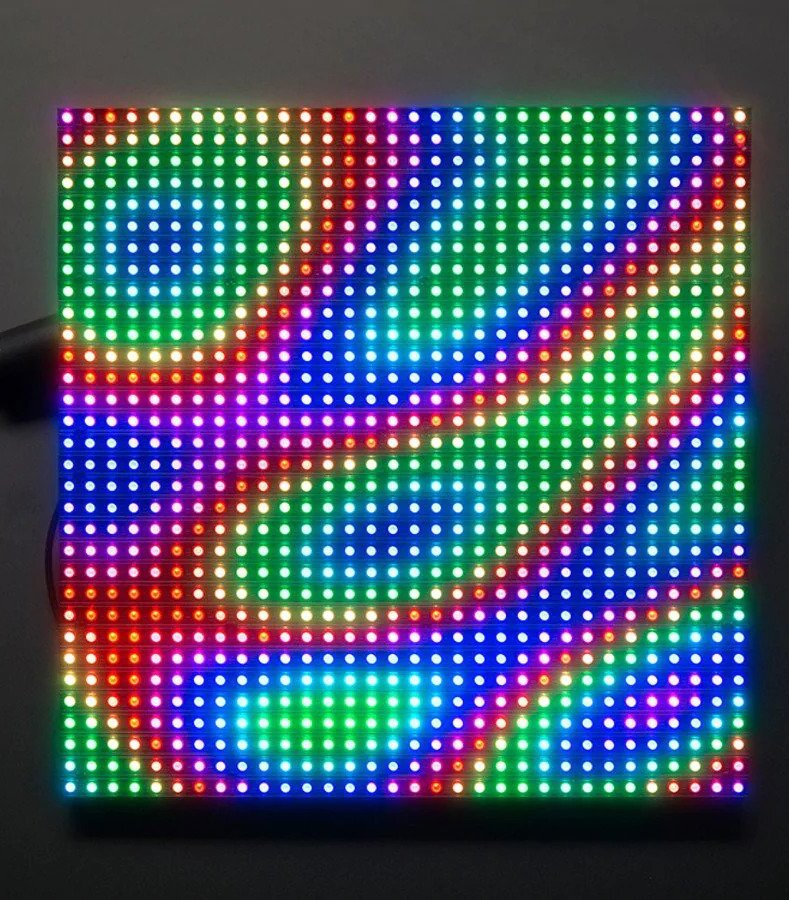
\includegraphics[height=\textheight - 13pt]{pictures/led-matrix-example}
		\end{tabular}
		& \parbox{0.5\linewidth}{
			\emph{Led Matrix}
			\begin{itemize}
				\item 64x64 Led Raster
				\item Erweiterbar
			\end{itemize}
		}
	\end{tabular}
	\customcite{led-matrix-example}
\end{frame}

\section{Problemstellung}

\begin{frame}{Problemstellung}
	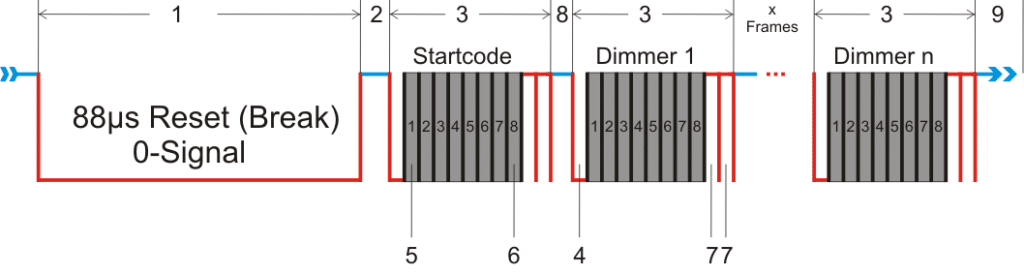
\includegraphics[width=\textwidth]{pictures/dmx-timing}
	\begin{itemize}
		\item DMX Protokoll in Datenblättern erklärt
		\item Demo Projekt für Lehre fehlt
	\end{itemize}
	\customcite{dmx_timing}
\end{frame}
\begin{frame}{Problemstellung}
	\begin{tabular}{cl}  
		\parbox{0.45\linewidth}{
		\emph{Forschungsfragen}
		\begin{itemize}
			\item Wie kann das Protokoll am besten heruntergebrochen werden?
			\item Welche Darstellungsformen eignen sich?
			\begin{enumerate}[label=\arabic*.,start=\value{enumi}]
				\item[$\rightarrow$] Kanal Abbildung/ Parametrisierte Animationen
			\end{enumerate}
			\item Evaluierung des Lerneffekts
		\end{itemize}
		}
		&
		\begin{tabular}{c}
			
\includegraphics[height=\textheight - 13pt]{pictures/oder}
		\end{tabular}
	\end{tabular}
	\customcite{fragen}
\end{frame}
\begin{frame}{Problemstellung}
	\begin{tabular}{cl}  
		\parbox{0.45\linewidth}{
			\emph{To Do}
			\begin{itemize}
				\item[\checkmark] Led Matrix Treiber
				\item[$\times$] DMX Slave Treiber
				\item[$\times$] Raspberry Pi Hat Platine
				\item[$\times$] DMX Protokoll Visualisierung
				\item[$\times$] Gehäuse
			\end{itemize}
		}
		&
		\begin{tabular}{c}
			\includegraphics[height=\textheight - 13pt]{pictures/Problemstellung}
		\end{tabular}
	\end{tabular}
	\customcite{problemstellung}
\end{frame}

\section{Methodik}

\begin{frame}{Methodik}
	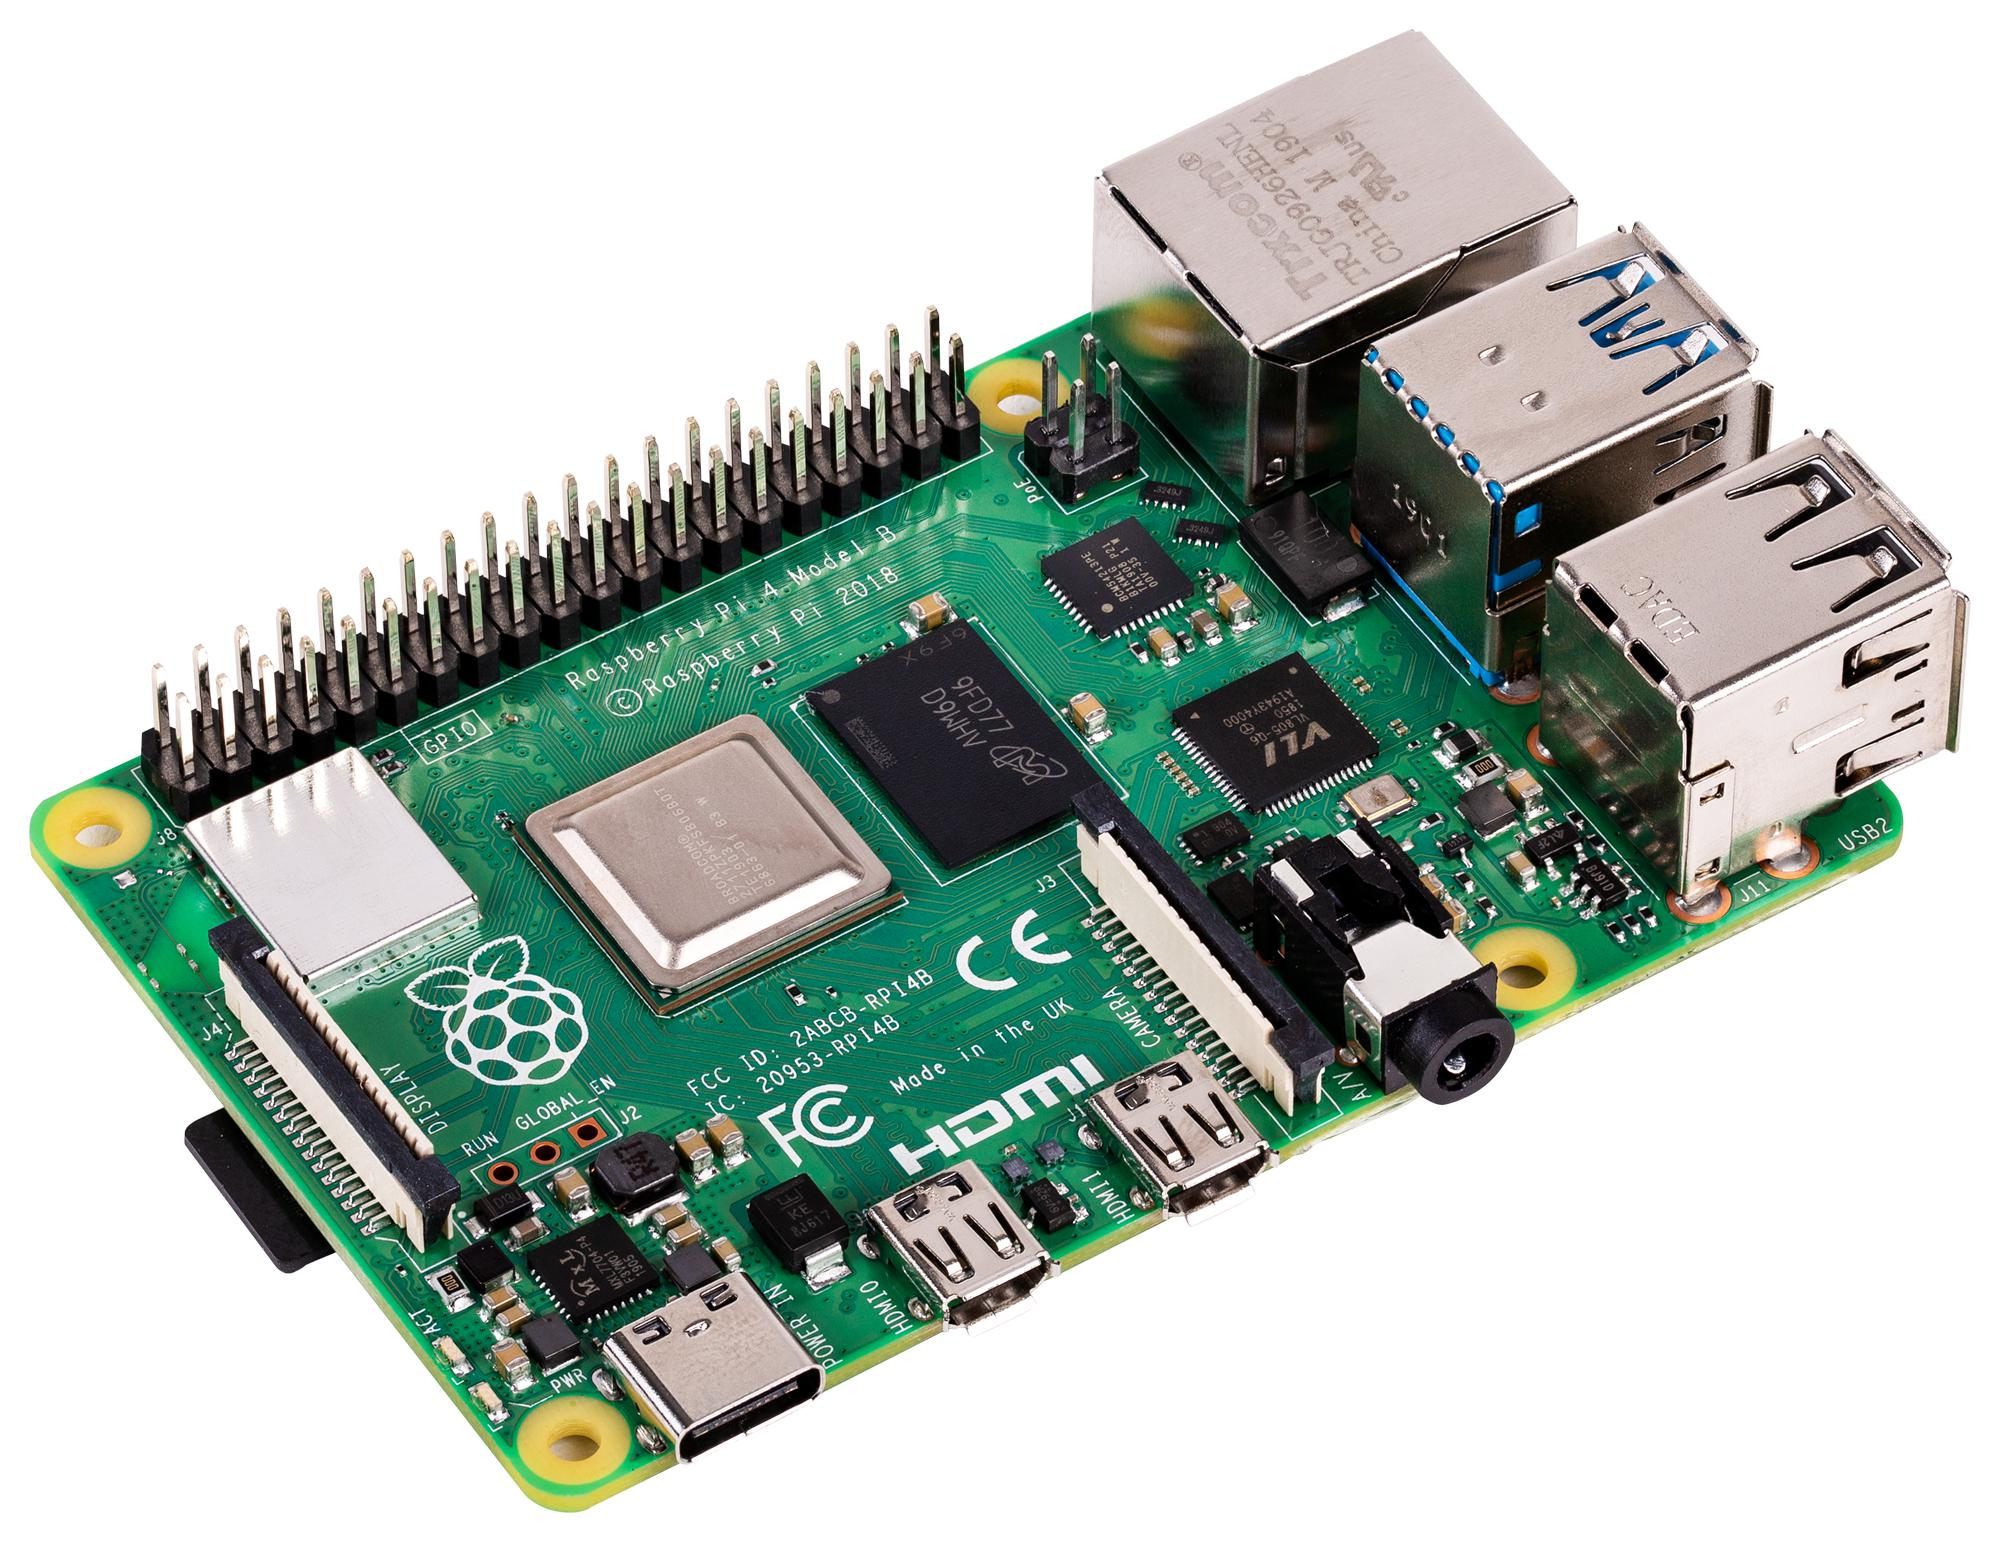
\includegraphics[scale=0.05]{pictures/rpi}
	\scalebox{-1}[1]{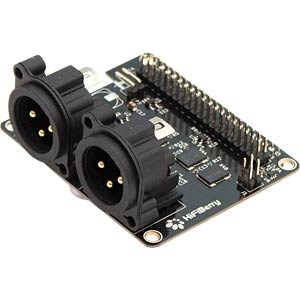
\includegraphics[scale=0.3]{pictures/rpi-hat}}
	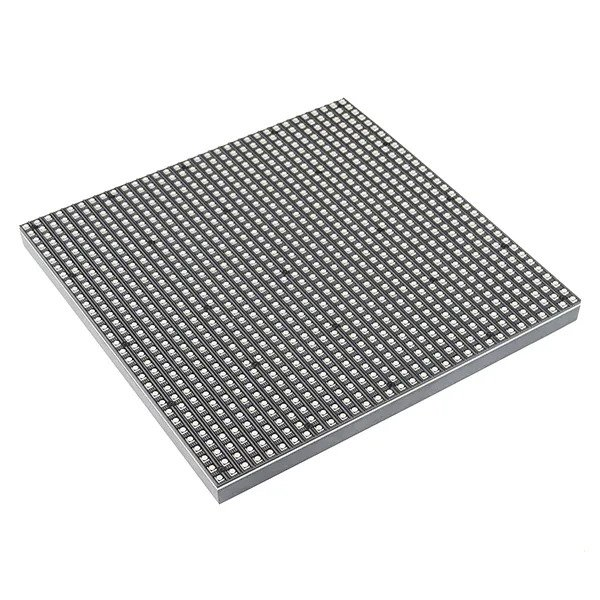
\includegraphics[scale=0.2]{pictures/led-matrix}
	\begin{itemize}
		\item Platform: Raspberry Pi
		\item Eigene RPi HAT Platine
	\end{itemize}
	\customcite{rpi, rpi_hat, led_matrix}
\end{frame}

\section{Zeitplan}

\begin{frame}{Zeitplan}
	\begin{center}
		\begin{tabular}{ | c | *{6}{c} | }
			\hline
			\multirow{2}{*}{Zeitplan}\ & \multicolumn{6}{c | }{Woche} \\ 
			& 1-3 & 4-6 & 7-9 & 10-13 & 14-17 & 18-20 \\
			\hline
			LED Matrix Ansteuerung		& x & & & & & \\
			LED Matrix Animationen		& & x & & & & \\
			DMX Kanäle/ Paket Visualisierung		& & x & & & & \\
			\hline
			Raspberry Pi DMX Treiber	& x & & & & & \\
			Raspberry Pi HAT Platine	& & x & & & & \\
			Gehäuse									& & & x & & & \\
			\hline
			Projekt Dokumentation			& & & x & & & \\
			Evaluierung								& & & & x & & \\
			Rohtext verfassen					& & & & x & x & \\
			Feedback \& Überarbeitung		& & & & & x & x \\
			Schlusskorrektur					& & & & & & x \\
			Abgabe										& & & & & & x\\
			\hline
		\end{tabular}
	\end{center}
\end{frame}

\begin{frame}{Quellen}
\bibliographystyle{unsrtnat} % Use the "unsrtnat" BibTeX style for formatting the Bibliography
\nocite{cover, banner}
\scriptsize
\bibliography{Bibliography}
\end{frame}
\begin{frame}{Danke}
	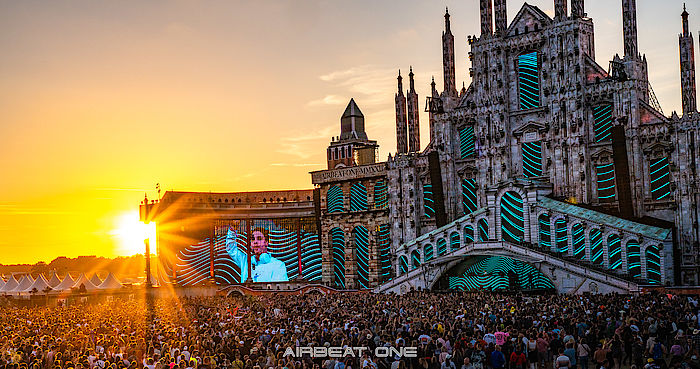
\includegraphics[width=\textwidth - 13pt]{pictures/led-matrix-beispiel}
	\customcite{led_matrix_lightshow}
\end{frame}

\end{document}
